%%%%%%%%%%%%%%%%%%%%%%%%%%%%%%%%%%%%%%%%%%%%%%%%%%%%%%
 \begin{figure*}[h] 
    \subfloat[Stage-wise breakdown]
    {
    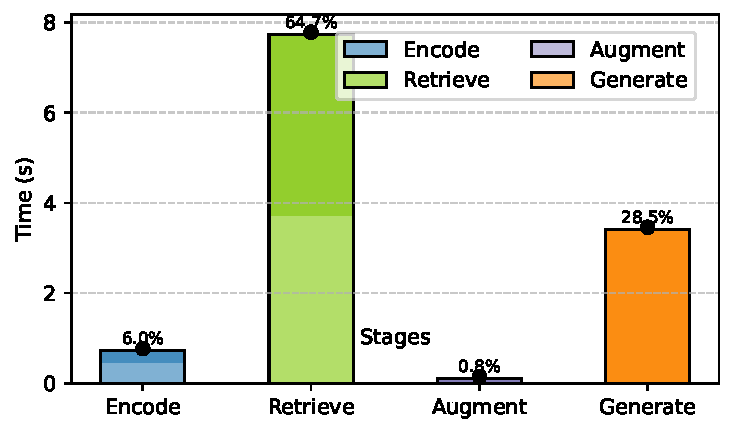
\includegraphics[clip,width=0.3\linewidth, height=1in]{Figs/stacked_graph.pdf}%
    \label{Fig:stacked_graph}
    }
    \hfill
    \subfloat[Encoding latency vs batch size scaling]
    {%
    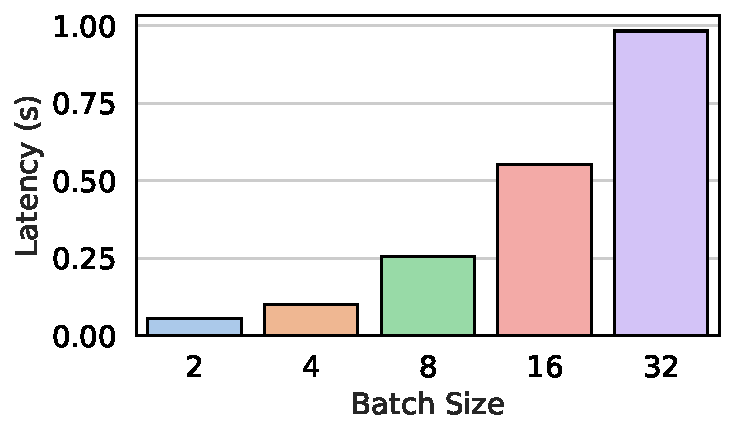
\includegraphics[clip,width=0.3\linewidth, height=1in]{Figs/forwardpass_8cores.pdf}%
    \label{Fig:forwardpass_8cores}
    }
    \hfill
    \subfloat[Encode latency vs core scaling]
    { 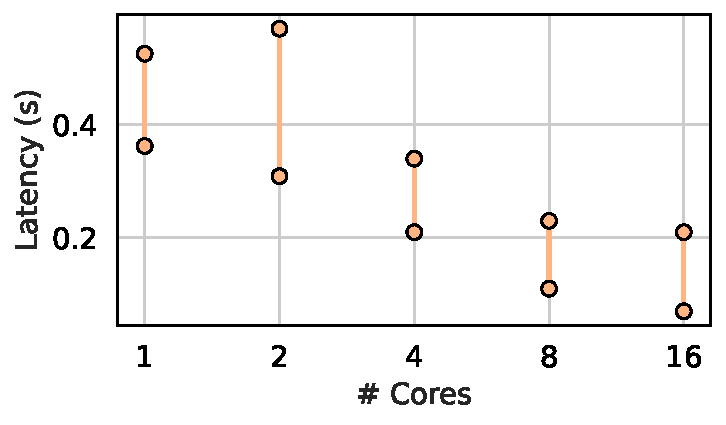
\includegraphics[clip,width=0.3\linewidth, height=1in]{Figs/forwardpass_bs16_range_discrete.pdf}%
    \label{Fig:forwardpass_bs16_range_discrete}
    }

    
    \subfloat[Batch Size vs Latency in RTX 4090]
    {%
    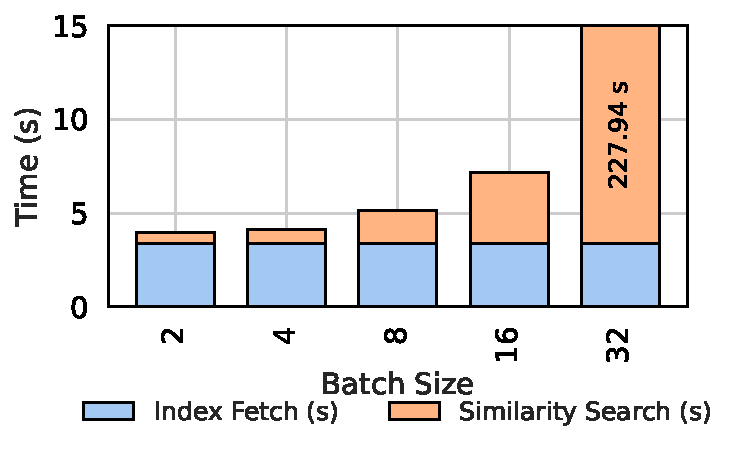
\includegraphics[clip,width=0.3\linewidth, height=1in]{Figs/batchsize_stacked_linear_labeled.pdf}%
    \label{Fig:batchsize_stacked_linear_labeled}
    }
    \hfill
    \subfloat[\# Cores vs Latency in RTX-4090]
    {%
    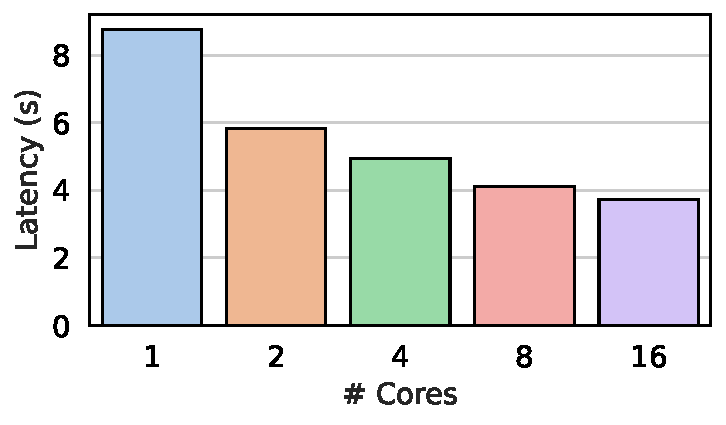
\includegraphics[clip,width=0.3\linewidth, height=1in]{Figs/latency_cores.pdf}%
    \label{Fig:latency_cores}
    }
    \hfill
    \subfloat[DB Size vs Latency in RTX 4090]
    {%
     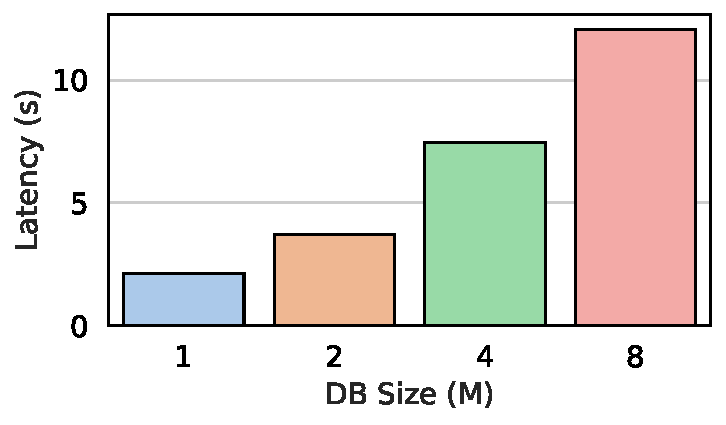
\includegraphics[clip,width=0.3\linewidth, height=1in]{Figs/latency_dbsize.pdf}
    \label{Fig:latency_dbsize}
    }
    \caption{Characterizations: 
    (a) Stage-wise breakdown of RAG pipeline. Lighter shades represent start-up cost and darker execution time. Characterization for \textbf{encode stage} 
    (b--c): 
    (b) Encode stage latency for different batch sizes on 8 cores.
    %At low core counts, concurrency helps significantly, but overheads grow after about 8 cores. 
    (c) Encode latency at batch size 16 as we vary the number of CPU cores. 
    %Execution scales well until roughly 16 queries, after which overheads grow faster. 
    Characterization for \textbf{retrieval stage} (d--f):
    (d) Retrieval stage breakdown on 4 cores with different batch sizes (\emph{Index Fetch} vs. \emph{Similarity Search}).
    %Adding more cores steadily reduces latency, but the returns diminishes at higher core counts. 
    (e) Retrieval latency as the number of CPU cores increases (DB size = 2\,M, batch size = 8). 
    %Doubling DB size has near-linear impact on retrieval time, highlighting the I/O-bound nature of the search. 
    (f) Retrieval latency vs. database size (batch size = 8).
    %For medium batch sizes (8--16), overheads stay balanced, but very large batches cause memory thrashing and high search time.
    }
    %\vspace{-0.1cm}
    \label{Fig:FwdPass4090}  
    \vspace{-10pt}
\end{figure*}
%%%%%%%%%% %%%%%%%%%% %%%%%%%%%% %%%%%%%%%%
%%%%%%%%%% %%%%%%%%%% %%%%%%%%%% %%%%%%%%%% 
\section{Detailed Characterization}
\label{sec:03Characterization}

% Text matter begin
%%%%%%%%%% %%%%%%%%%% %%%%%%%%%% %%%%%%%%%% 
This section characterizes the performance of a RAG pipeline on a desktop-class machine, highlighting how resource allocation, database size, and batching affect each stage. Our experiments use an Intel i9-14900K processor (24 physical cores), 128\,GB RAM, and an RTX 4090 GPU~\cite{intel_cpu,nvidia_rtx_gpu}, with the generation length fixed at 120 tokens. To analyze performance bottlenecks, we decompose the pipeline into four stages—\emph{encode}, \emph{retrieve}, \emph{augment}, and \emph{generate}—each with distinct computational and memory demands (further detailed in \Cref{sec:04Design}). The first three stages run on the CPU, while generation executes on the GPU. \Cref{Fig:stacked_graph} shows the stage-wise execution time for a batch of 8 queries accessing a 4M-entry database, where each knowledge element consists of approximately 100 words. For this baseline, encoding, retrieval, and augmentation are run on a single CPU core to compare their compute cost.

\subsection{Encoding Stage}
\label{sec:char:Encoding}
The encoding stage converts user inputs into high-dimensional embeddings, with latency influenced by both batch size (\texttt{BS}) and available compute resources. \Cref{Fig:forwardpass_8cores} shows that increasing \texttt{BS} over a fixed number of CPU cores (8 P-cores) leads to higher latency due to increased workload. While scaling the number of cores reduces latency, this benefit quickly saturates. \Cref{Fig:forwardpass_bs16_range_discrete} shows diminishing returns beyond 8 cores. These results show that allocating extra cores help only for sufficiently parallel workloads.% (e.g., \texttt{BS=32}).

\subsection{Retrieval Stage}
\label{sec:char:Retrieval}
The retrieval stage performs a similarity search over a vector database to identify the \topk relevant entries. As a predominantly I/O- and memory-bound phase, it demands detailed characterization to expose performance bottlenecks. Retrieval comprises two components: (i) index fetch, which occurs once per batch and is independent of batch size, and (ii) similarity search, which runs per query. \Cref{Fig:batchsize_stacked_linear_labeled} shows that index fetch dominates latency at small batch sizes, while similarity search grows with \texttt{BS} and becomes dominant at larger batches. At \texttt{BS=32}, total latency increases sharply due to DRAM bandwidth saturation.
\Cref{Fig:latency_cores} shows sub-linear latency reductions as CPU cores are increased, suggesting diminishing returns from parallelism. By contrast, \Cref{Fig:latency_dbsize} reveals near-linear latency growth with database size, indicating stronger sensitivity to memory and I/O bandwidth than to core count. Overall, retrieval latency is governed more by data movement and cache behavior than raw compute.

% --------------------------------------------------------------------
%  Execution, Batch/Core, DB-size, and Key Observations
% --------------------------------------------------------------------

\noindent\textbf{Execution Breakdown Across Stages:} 
\Cref{Fig:latency_cores} shows that adding CPU cores shortens retrieval latency up to 8 cores, after which benefits plateau because shared‐resource pressure, i.e. memory bandwidth and LLC capacity, dominates.  
\Cref{Fig:batchsize_stacked_linear_labeled} further decomposes retrieval into \emph{index fetch} (I/O-bound, once per batch) and \emph{similarity search} (compute-bound, per query).  
At small batches, fixed I/O cost dictates latency; at larger batches, similarity search and DRAM contention take over, revealing that retrieval performance is governed primarily by the memory hierarchy, with compute parallelism offering only secondary gains.

\noindent\textbf{Impact of Batch Size and Multicore Scaling:} 
\Cref{Fig:forwardpass_8cores} illustrates that encoding enjoys linear core-utilization only when the batch size (\texttt{BS}) is large enough to saturate all cores.  
However, pushing \texttt{BS} beyond 16 inflates the working-set footprint, increasing cache evictions and risking DRAM thrashing; in retrieval the same threshold (\Cref{Fig:batchsize_stacked_linear_labeled}) triggers bandwidth saturation.  
Thus, while larger batches amortize per-query overheads and improve throughput, they must be balanced against memory-hierarchy limits to avoid super-linear latency growth.

\noindent\textbf{Effects of Database Size:} 
\Cref{Fig:latency_dbsize} shows nearly linear latency growth as the vector store expands from 1 M to 8 M entries on 16 cores.  Once the index outgrows the cache capacity ($\approx30 MB$) and approaches DRAM, miss penalties and page faults dominate, diminishing the marginal benefit of additional cores.  Hence, scaling the database, without architectural support such as tiered caching or sharding, yields a proportional increase in retrieval time, confirming that I/O, not compute, is the principal bottleneck for large knowledge stores.

%%%%%%%%%% %%%%%%%%%% %%%%%%%%%% %%%%%%%%%% 
\begin{figure*}[!ht] 
    \subfloat[Latency-critical pipeline]
    {%
     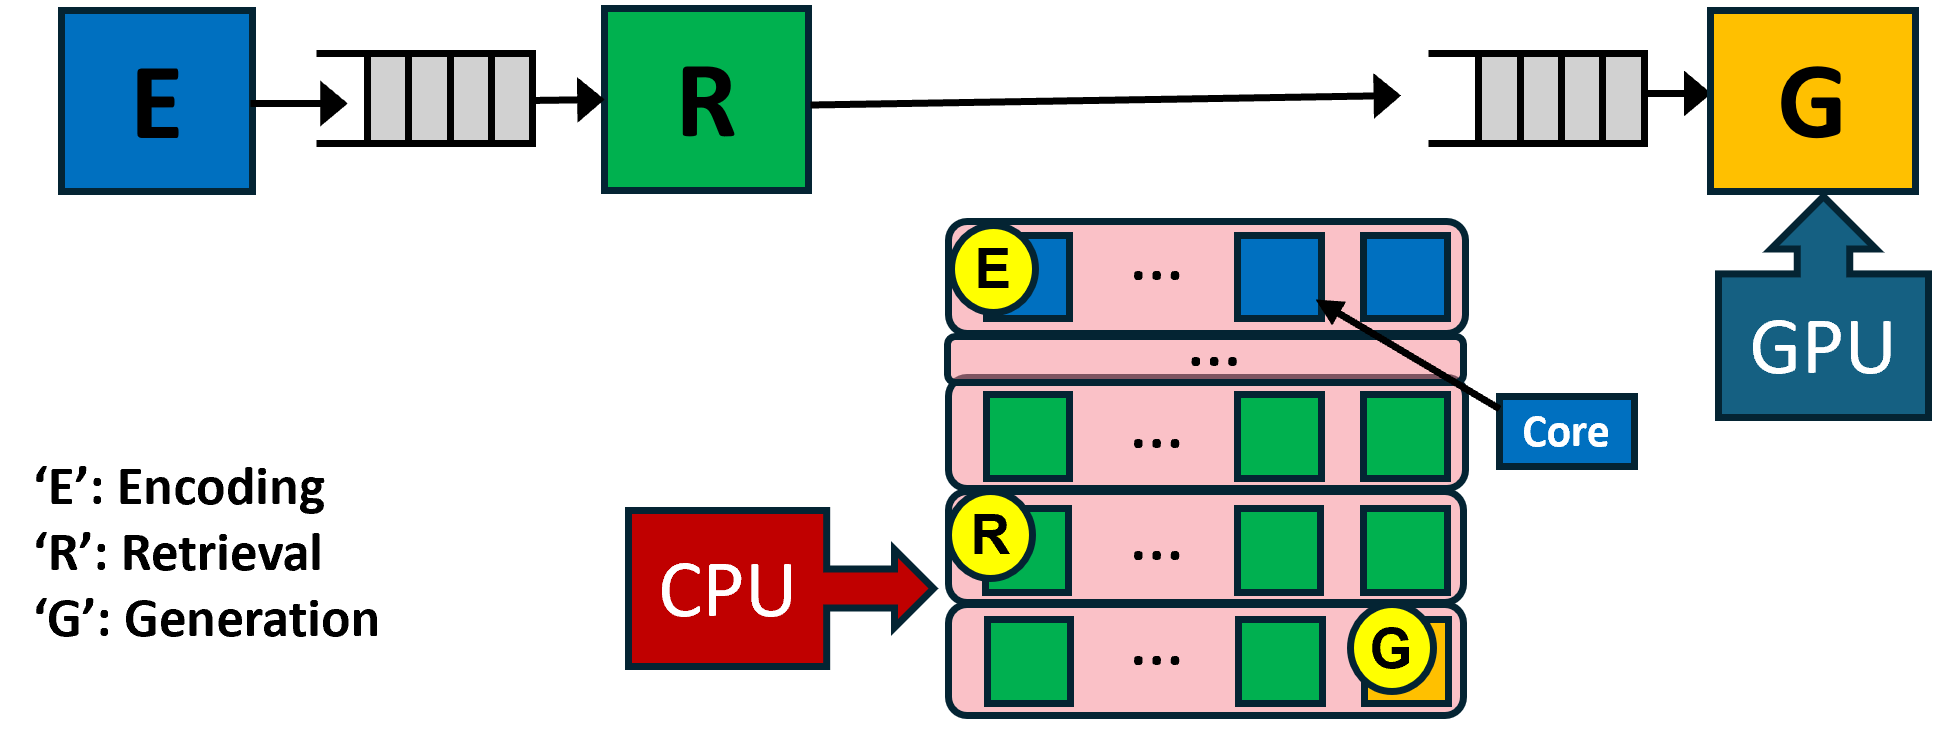
\includegraphics[clip,width=0.32\linewidth]{diagrams/latency_oriented_pipeline.png}%
    \label{fig:latency_oriented_pipeline}
    }
    \hfill
    \subfloat[Throughput-critical pipeline]
    {%
    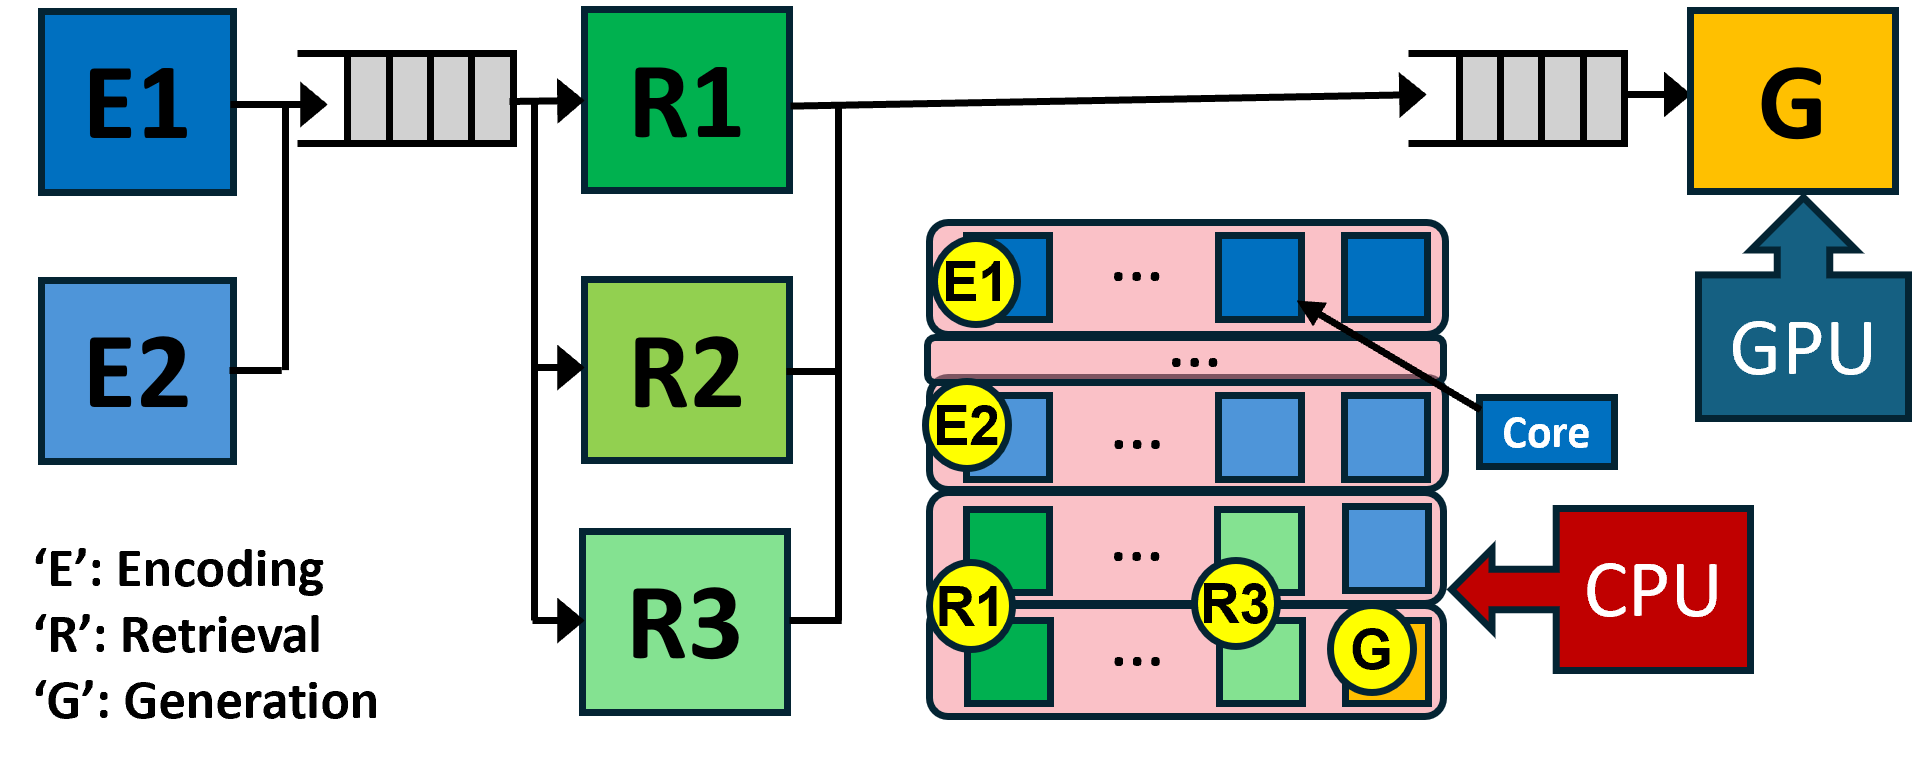
\includegraphics[clip,width=0.32\linewidth] {diagrams/throughput_oriented_pipeline.png}%
    \label{fig:throughput_oriented_pipeline}
    }
    \hfill
    \subfloat[\design{} pipeline vs others]
    {%
    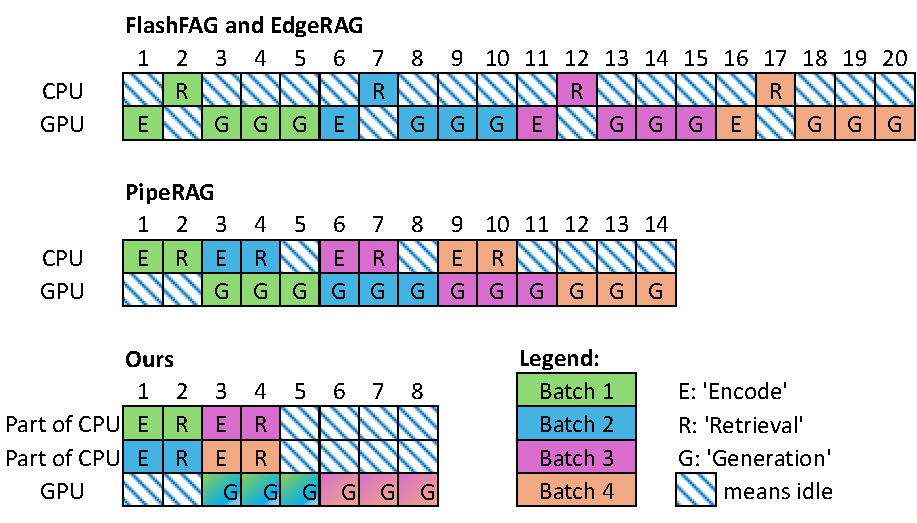
\includegraphics[clip,width=0.32\linewidth] {diagrams/pipeline_comparison_schematic.pdf}%
    \label{pipeline_comparison_schematic}
    }
    \caption{\design{} pipeline: (a) latency-critical pipeline has a minimum number of parallel workers in each stage to maximize the number of CPU cores per stage. (b) throughput-critical pipeline has more number of parallel workers in the encode and retrieve stages to maximize the number of batches being processed. (c) Pipeline representation comparing prior works with \design{}, where multiple batches are executed on the same hardware platform (both CPU and GPU).}
    %\vspace{-0.1cm}
    \label{Fig:OurPipelines}  
    \vspace{-10pt}
\end{figure*}
%%%%%%%%%% %%%%%%%%%% %%%%%%%%%% %%%%%%%%%%

\subsection{Key Observations and Motivation for Design}
Encoding remains mostly compute-bound and scales with moderate core counts, whereas retrieval is tightly coupled to memory bandwidth and database footprint, exhibiting diminishing returns from both batching and additional cores.  
Augmentation is lightweight and benefits from being fused with retrieval to avoid extra copies.  
Generation is GPU-bound but stable unless models are frequently reloaded or prompts become excessively long.  
Therefore, effective pipeline orchestration requires:  
(i) judicious CPU-core allocation between encoding and retrieval,  
(ii) batch sizing that maximizes utilization without breaching cache/DRAM limits, and  
(iii) selective offloading, only stages whose compute time exceeds transfer overheads, should migrate to the GPU.  
These insights inform the multi-stage scheduling strategy introduced in \Cref{sec:04Design}.

%%%%%%%%%% %%%%%%%%%% %%%%%%%%%% %%%%%%%%%%
% \noindent\textbf{Execution Breakdown Across Stages:} 
% \Cref{Fig:latency_cores} shows that increasing CPU cores reduces retrieval latency, but the speedup is sub-linear due to contention in shared resources such as memory bandwidth and last-level cache. Beyond 16 cores, gains diminish, reflecting that retrieval is constrained more by I/O throughput than by raw compute.

% \Cref{Fig:latency_dbsize} illustrates that retrieval time scales nearly linearly with database size—from 1\,M to 8\,M entries—as larger indices exceed LLC (Last Level Cache) capacity, leading to more frequent cache misses and reliance on slower DRAM access. Since index structures exhibit limited temporal locality across queries, reuse in cache is poor, especially under large batch sizes or when the working set exceeds DRAM page cache.

% \Cref{Fig:batchsize_stacked_linear_labeled} provides further insight into this trend: at small batch sizes, index fetch dominates latency due to repeated I/O reads with minimal amortization. As batch size grows, similarity search becomes more prominent, and the system may saturate DRAM bandwidth, compounding latency. Overall, these results indicate that retrieval latency is primarily shaped by memory hierarchy limits and database footprint, with only moderate benefits from compute parallelism.


% %\subsection
% \noindent\textbf{Impact of Batch Size and Multicore Scaling:} 
% ~\Cref{Fig:forwardpass_8cores} shows how encoding time scales with batch size on 8 CPU cores. Although small batch sizes observe lower latency compared to larger batch sizes, they do not fully utilize CPU resources. However, larger batches risk higher memory footprints and potential thrashing. In retrieval, these tradeoffs manifest in \Cref{Fig:batchsize_stacked_linear_labeled}, where going beyond a batch size of 16 significantly inflates total execution time, partly because the system expends more time on either index fetching or computing similarities for many queries in one go. 

% \noindent\textbf{Effects of Database Size:}
% \Cref{Fig:latency_dbsize} demonstrates how the retrieval latency scales with the size of the DB on 16 CPU cores. Increasing from 1\,M to 2\,M entries roughly doubles the time, and at 8\,M entries, we see further linear growth. While more CPU cores can mitigate retrieval cost to a degree, the cost of scanning a large index remains partly I/O-bound. As a result, simply adding cores does not proportionally reduce the penalty incurred by a growing database.


% \subsection{Key Observations and Motivation for Design}
% We observe that encoding scales well with moderate core counts and remains mostly compute-bound, while retrieval is especially sensitive to memory footprint and I/O activity, causing diminishing returns as the batch size grows. Augmentation is lightweight and best merged with retrieval to avoid extra data transfers. Although GPU-based generation can be the longest stage, its runtime often remains stable unless the model is repeatedly reloaded or the prompts are excessively large. Consequently, it becomes crucial to allocate CPU cores judiciously for encoding and retrieval and to prevent ballooning memory usage at high batch sizes or large databases. Furthermore, offloading the encoder to the GPU can be inefficient when transfers dominate, emphasizing the importance of selectively assigning each stage to CPU or GPU. These insights form the basis for our multi-stage pipeline and scheduling in \Cref{sec:04Design}.

                                     
%%%%%%%%%% %%%%%%%%%% %%%%%%%%%% %%%%%%%%%% 
% Text matter end

% \section{RAG Pipeline Execution Characterization}
% \label{sec:characterization}
% This section conducts a detailed profiling study and provides various system and architecture level insights into the RAG pipeline and the factors influencing performance across different stages. As mentioned in Section~\ref{sec:background}, since each RAG stage differs in its computational and IO needs, we characterize each stage individually to understand its system level needs. We choose CPU as the hardware of choice to profile the first two stages --retrieve and augment-- to closely monitor the utilization and memory needs. 


% \subsection{RAG Inference using CPUs and GPU:}
% Figure. \ref{fig:pipeline} depicts the sequence of events in pipeline diagram for the cases of intra-batch \circled{1} and inter-batch \circled{2} execution. As mentioned earlier, GPU is used for executing two stages: encoding and generation. When processing an input batch, we note three key communication  between the CPU and the GPU: (1) loading of the LLM on GPU (2) after encoding stage, there is transfer of intermediate embedding vectors from GPU to CPU (3) for generation stage, the augmented prompt is transferred from CPU to GPU. Across batches, each encoding in a batch is preceded by loading the LLM. For generation stage, Fig.~\ref{fig:model_loading} shows the time taken to load and initialize different models. Our profiling shows that it takes a significant time of 2.27 seconds for initializing the Llama3 8B model. 


% We note that due to resource constraints and contention on personal computing platforms having a single GPU, it is not possible to fully overlap computations across batches in a pipelined manner. With a mix of compute intensive and high IO operations happening within and between both CPU and GPU with different hierarchies of memory involved, RAG presents itself as a complete architectural problem waiting to be understood. Since the architectural level implications of this application have been explored sparsely, we start with breaking down the pipeline and study each stage in detail. Thus, we explore the hidden architectural implications that these different stages of RAG pipeline have in detail to find an optimal pipeline orchestration strategy which would reduce the costly IO at the same time have lesser penalty towards latency.


% \subsection{Execution Breakdown Study}
% Fig. \ref{fig:execution_breakdown} shows the breakdown of the execution time of different stages of RAG pipeline to process one batch comprising of 8 queries retrieving 5 knowledge points each from a database of 2 million knowledge points having flat indexing. We fix the core per stage to one so as to get the ratio of execution times in an iso-resource situation. The retrieval and augmentation stages are run on CPU while the  generation stage is run on GPU. There exist works~\cite{gpuchar, gpuchar1, gpuchar2} that have precisely characterized the execution of LLM on different devices and positioned GPUs to be the better contender compared to CPU. Taking that into account, we run the last generation stage on the available GPU resource. We break open the retrieval stage and partition it into two sub-stages having different system characteristics: i) Encode ii) Retrieval. The encode stage here refers to the conversion of textual prompts into higher dimensional embedding vectors through an embedding model. The retrieval stage on the other hand refers only to the subsequent similarity search of this input prompt embedding vector in the database and giving back top 'k' most similar embedding vectors as output.

% We observe that the execution of this pipeline is severely imbalanced where the encode stage takes majority of time ($\approx$ 84.70\%) followed by the retrieval stage ($\approx$ 8.43\%). The generation stage contributes to $\approx$ 6.7\% of entire end-to-end pipeline execution latency. The augmentation stage, which only does data stitching, is the least computationally heavy stage,  contributing to 0.18\% of pipeline execution time. The associated execution times are 47.8s, 4.8s, 3.8s, and 0.1s for encoding, retrieval, generation, and augmentation stages respectively. Note that an optimization strategy like "pipelining" --to ensure requests are overlapped in execution-- would be little effective here since the inherent imbalance of this pipeline would introduce "pipeline bubbles", causing hardware resources to be underutilized. One way to move about is to dissect into the computational and memory needs of these stages to find whether the execution times of each stage are due to the computational complexity or IO latency. Since the encode and retrieve are the stages performed on CPU having significant contribution to end-to-end execution time, the next subsection studies their multi-core scaling behavior. 


% \subsection{Multi-core Scaling Study}
% Fig. \ref{fig:encode_stage_core_util_study} and Fig. \ref{fig:retrieval_stage_core_util_study} shows the execution time and utilization variation as the number of cores for the encode and retrieve stages increase. We observe that, as the number of cores is increased for encode stage, the execution time drops progressively while the average core utilization remaining high, indicating that it is a compute intensive stage. In contrast, with the increase in the number of cores, the retrieve stage's execution time drops less rapidly while the utilization drops more rapidly, indicating less benefit as we provision more CPU cores to it. 

% \subsection{Impact of Workload Properties on Execution}
% As shown in \Cref{fig:encode_stage_batch_size_study}, when we increase the number of requests in a batch in the encode stage, we see a corresponding increase in the execution time across different number of cores given to perform the task. We observe that the difference in the execution time of encode for different batch sizes is more significant in cases with fewer cores. This further validates our previous observation of the encode stage being a computationally heavy stage, which scales with the amount of work and the hardware resource provided. Similarly, in the retrieve stage, as depicted in \Cref{fig:retrieval_stage_1core_study}, the execution time increases with the batch size, implying that the amount of task being a contributing factor for the execution time. \Cref{fig:retrieval_stage_1core_study} also shows that the number of retrieved elements exhibits small variations with the number of retrieved knowledge points. 


% \subsection{Motivation}
% With these insights, we qualitatively evaluate the state of the art solutions and identify optimization opportunities targeting end-to-end pipeline. In works like FlashRAG~\cite{jin2024flashrag}, we see the initial prompt encoding stage taking place on GPU, followed by retrieval and augmentation tasks scheduled on CPU. The generation stage is done on GPU, which starts with loading the generation model followed by loading the structured prompts. While this solution might sound appealing for an enterprise-grade deployment where CPUs are provisioned with multiple GPUs so that the prompt encoding and the final generation can happen on two devices without incurring the penalty of loading model for each batch, it is not as attractive for personal compute platforms like laptops, desktops and mobile phones that are typically equipped with one GPU. This robs the user of the possible pipelining opportunity owing to resource contention and not being able to overlap of computation across successive batches to increase device utilization. On the other hand, PipeRAG~\cite{jiang2024piperag} attempts to bridge this gap, but it does not opportunistically schedule tasks on the available hardware to fully utilize the capacity of the CPUs.

%%%%%